\documentclass[11pt]{article}
\usepackage[margin=0.75in]{geometry}
\usepackage{amsmath}
\usepackage{physics}
\usepackage{listings}
\usepackage{caption}
\usepackage{graphicx}
\usepackage{algorithm}
\usepackage{algpseudocode}
\usepackage{setspace} \doublespacing
\usepackage{titling}
\graphicspath{{../Images/}}


\title{Emergence of Autocatalytic Reaction Networks}
\author{Varun Varanasi \\{Advisor: Jun Korenaga}}
\begin{document}

\maketitle
\newpage

\tableofcontents

\newpage

\section{Abstract}

Origin of life research is heavily focused on bridging the knowledge gap between prebiotic synthesis and emergence of life. 
Theoretical models posit that this transition was facilitated through a series of chemical reactions characterized by their ability to self-replicate, self-sustain, self-assemble, and autocatalyze.
Given the scarcity of known abiotic autocatalytic reactions, research efforts are focused on studying the emergence of autocatalysis in prebiotic chemical systems. 
Previous research has found a phase transition in the probability of producing an autocatalytic set in a kauffman model as a function of expected number of catalyzations, but details about the dynamics and characterization of this phenomena still remain an open question.
The goal of this research is to elucidate this relationship and develop a more cohesive understanding of autocatalytsis in prebiotic chemistry.
In particular, this work focused on mapping network properties and graph characteristics to the presence of autocatalytic sets. 
In addition, this work tested and the stability and robustness of autocatalytic sets in existing network models by inducing random catalytic perturbations.
The results of these tests found that graph proximity to the food set and presence of two-cycles in reaction networks are highly indicative of autocatalytic sets.
Furthermore, we see that this relation is inversely proportional to graph size. 
Perturbation analysis reveals to us that large networks are relatively more stable and that pertrubations based on the food-set are more influential at small sizes.
Results produced in this paper lay the groundwork for further testing that must be done to truly quantify and understand the true dynamics and constitution of the emergence of autocatalytic sets in kauffman models. 

\newpage

\section{Introduction}

\subsection{Motivation}


At a high level, my work this semester can be classified as origin of life research  falling under the larger umbrella of theoretical biology and prebiotic geophysics.
A complex and multifaceted mystery, we can break down the origin of life or abiogenesis into three rough phases. \\

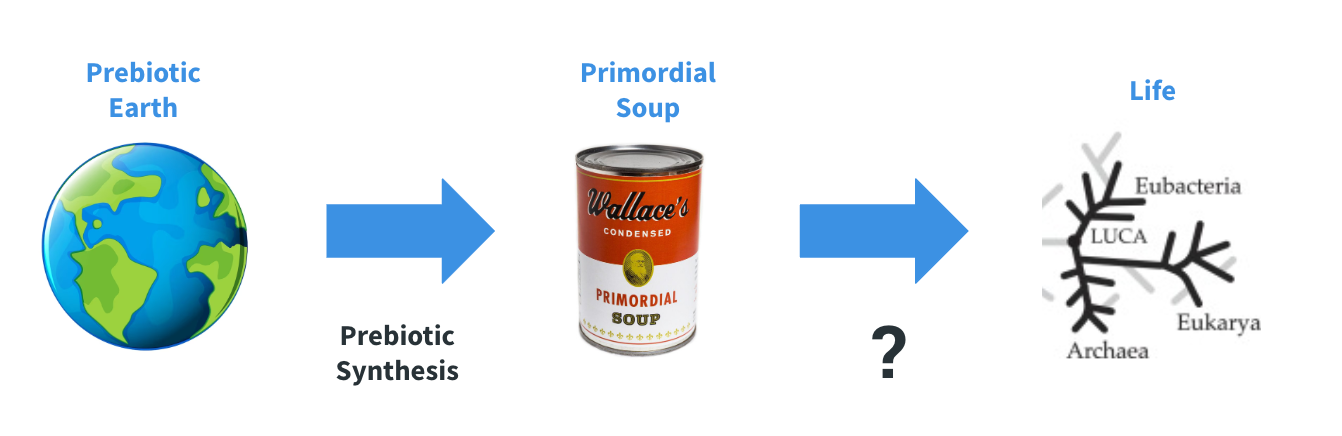
\includegraphics[width=\textwidth]{origin_of_life}

The first phase, labeled the Prebiotic Earth phase, occured approximately 4 billion years ago before life formed on Earth.
Still largely covered by liquid water, the Earth at this time was approximately 30\% dimmer than today with more x-ray and ultraviolet radiation.
The composition and chemistry of this time period still remains an open research question, but current theories characterize it as a weakly reducing atmosphere with an abundance of carbon dioxide and nitrogen, but very little oxygen.
All together, the conditions created an environment that was conducive to frequent ionization and an unstable atmosphere. \\

Over time, through a process known as prebiotic synthesis, the prebiotic earth evolved into a stage we refer to as the primordial soup. Prebiotic synthesis is the process by which biotic molecules such as amino acids and other biological compounds are created from abiotic precursors.
For the longest time the mechanics and credibility of this process remained unanswered, but in 1953 Stanley Miller and Harold Urey were able to replicate prebiotic synthesis in a University of Chicago laboratory.
The experiment applied repeated sparks to a gas chamber of water, methane, ammonia, and hydrogen to simulate lightnining in a prebiotic atmosphere. 
At the end of the experiment they were able to recover over 20 amino acids, the building blocks of proteins. 
This ground breaking experiment provided strong evidence supporting the prebiotic synthesis theory. \\

Eventually as prebiotic synthesis occured and amino acids and other biological compounds accumulated, Earth's became a primordial soup that contained the essential building blocks of life floating around the largely water covered Earth.
Somewhere along the line, life emerged. However, the processes for this emergence still remains unanswered.
Prevailing scinetific theories suggest that life initially began with the support of proton gradients provided by hydrothermal vents.
Eventually, these supported organisms became LUCA or the Last Universal Common Ancestor from which all other organisms we know descended.  
Darwinian evolution provides us a strong understanding of this evolutionary process, but how LUCA and its precurosrs emerged from the primordial soup still remains a mystery.

My work focuses on answering this question. Theoretical models posit that these pseudo-supported life forms required a series of coupled self-sustaining, self-replicating, and autocatalyzing chemical reactions.
With the supoort of hydrothermal processes these reactions were eventually able to "evolve" into acutal life. 



\subsection{Background}

\subsubsection*{Autocatalysis}
My work and a large subset of origin of life research is focused on studying the process of autocatalysis. In particular, we want to understand its prevalence, the emergence, and dynamics so that we can understand how life came to be.

\begin{figure}[H]
    \centering
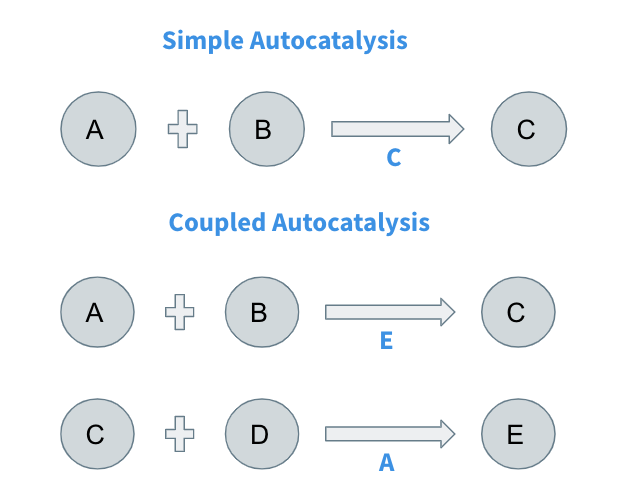
\includegraphics[width=8cm]{autocatalysis}
\caption{Autocatalysis}

\end{figure}

Autocatalysis, in its simplest definition, is a chemical reaction that is capable of catalyzing itself. 
In more general sitautions, autocatalysis can refer to a series of coupled reactions where each reaction is catalyzed by a product of another reaction in the reaction set. 
Autocatalytic reactions or autocatalytic sets function as positive feedback loops that are able to self-sustain and increase production as more products are produced. 
In the context of the origin of life, they are important in sustaining unfavorable chemical reactions and producing an abundance of molecular products required to produce life.

\subsubsection*{Reaction Networks}

Research is yet to discover an abiotic reaction capable of autocatalysis, so prebiotic autocatalysis research tends to focus on series of coupled chemical reactions. 
These systems are typically studied through reaction networks such as the one below. 

\begin{figure}[H]
    \centering
    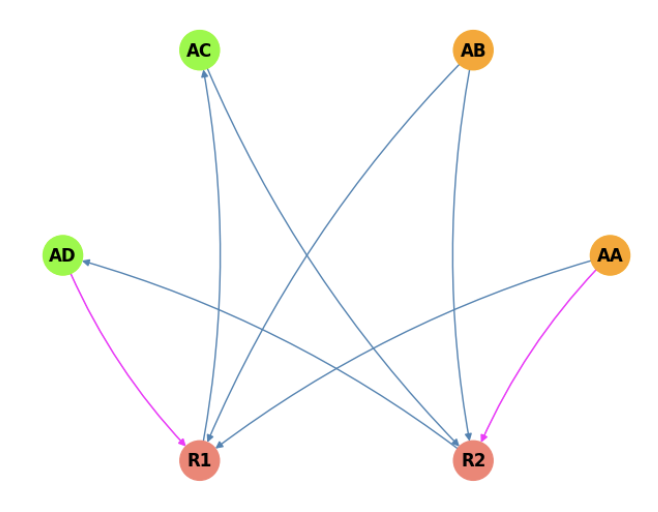
\includegraphics[width=8cm]{reaction_network}
    \caption{Reaction Network}
\end{figure}

We interpret the reaction network as follows. The yellow nodes represent the food set. These are the molecules that are ambient in the environment i.e. they do not need to be produced. 
The green nodes represent other molecules in a system. Finally, the red nodes represent reactions. Edges originating at a molecule vertex and ending at a reaction node represent the reactants of a given reaction.
Similarly, edges originating at a reaction node and ending at a molecule node represent a product. 
Putting it together, we see that R1 represents the reaction of $AA + AB \rightarrow AC$. 
The final details to note are the pink edges which represent catalyzation reactions. In the example above, we see that AD catalyzes R1 while AA catalyzes R2.
With this understanding in mind, we can begin to discuss the Kauffman model, our model for prebiotic chemistry. 


\subsubsection*{Kauffman Model}

The Kauffman model was developed by Stuart Kauffman in 1988 as a simplified representation of pre-biotic chemistry. 
Rather than focusing on actual chemical reactions, the essence of the model is to abstract chemical reactions into 4 sets of molecules and molecular relations.

\begin{itemize}
    \item X: The set of all possible molecules
    \item F: The set of food molecules
    \item R: The set of all possible reactions allowed
    \item C: The set of catalyzing relations
\end{itemize}

X, the set of all possible molecules, is typically defined by two paramters: t and n. t represents the size of the alphabet used in the model while n represents the maximum size of a molecule in our set. 
Therefore, X is the set of all possible configurations up to length n where each index takes t possible values.
Typically, t takes on the value of 2 which represents either a 0 or 1 in each index. Depending on the size of the model, n can take on a range of values. Therefore, most models have a total of $2^{n +1} -2$ molecules and as we increase n, the size of our model grows exponentially.
Next, F represents the food set. As explained above, the food set is a representation of ambient molecules in the environment. These are molecules that exist in a theoretical sink and can be used without replacement.
R is the set of possible reactions allowed. In the Kauffman model the allowed reactions are concatenation reactions and splitting reactions. In other words, if the joining of two molecules end to end produces another molecule in X, then that is a valid reaction.
Similarly, if we can split a molecule in X into two other molecules also in X we can define a splitting reaction.
The final component of the Kauffman model is C, the set of catalyzing reactions. Each reaction in R can be catalyzed by any molecule in X. Therefore, the size of C is given by $X \cross R$. 
Since X, F, and R are each static parameters defined by the model type, in our experiments we tend to vary C and study the resulting behavior.

\subsubsection*{Autocatalytic and RAF Sets}

The kauffman model provides us a framework for chemical reactions, but doesn’t tell us anything about our goal: autocatalytic sets. 
As we talked about earlier, autocatalytic sets are self-catalyzing reactions. 
Depending on how the catalyzation relations align, a given Kauffman network can potentially contain autocatalytic sets within it. 
To make our model more robust, we can further require that the reaction set is self-sustaining. In other words, in a given environment the autocatalytic set would be able to survive. 
One way of ensuring this is to make sure every molecule in the set is either from the food set (the set of ambient molecules) or produced by the food set through a catalyzed reaction.
 We call such a set RAF which stands for reflexively autocatalytic and food-generated set. 

\subsection{Previous Work}

Now, with our understanding of autocatalysis, reaction networks, the Kauffman model, and RAF sets we can quickly cover key results in the field.
Namely, we will discuss the discover of a phase transition in the probability of finding an RAF set in a given Kauffman model.
Published in 2004, "Detecting Autocatalytic, self-sustaining sets in Chemical reaction systems" by Hordjik and Steele details a novel algorithm to detect RAF sets in chemical reaction systems.

In their work they explore the probability of RAF occurence as a function of a probability parameter p. For a pre-defined p, each trial randomly creates a Kauffman network where each possible catalyzing reaction is included in C with probability p.
Based on this parameter p, they define a secondary value $f = |R| \cdot p$ which is a measure of the expected number of catalyzations per molecule.
For varying f values, Hordjik and Steele tested the probability of finding an RAF set for multiple values of n. 

\begin{figure}[H]
    \centering
    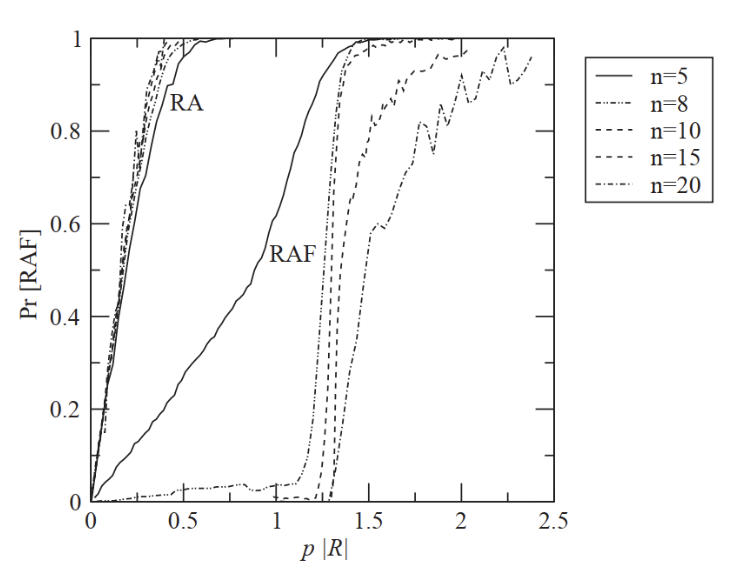
\includegraphics[width=15cm]{hordjik04}
    \caption{RAF Phase Transition}
\end{figure}

In particular, we see that at $f =1.25$ the probability of detecting an RAF set jumps from near 0 to apprximately 100\%. 
We also see that as n increases the steepness of this jump increases. 

\section{Classification}


\subsection*{Methodology}

The first task I set out to accomplish this semester was to replicate and verify the results produced by Hordjik and Steele. Funnily enough, this phase alone took me more than half the semester.
Given the groundwork laid out by Hordjik and Steele and my preliminary replication, we see that RAF emergence is strongly connected to expected number of catalyzations. 
The first question we asked was what else is the emergence of an RAF set correlated with? In other words, what are other important conditions in determining the presence of an RAF set?


To answer the posed question, our idea was to approach the problem as a classification problem. Given a sufficiently large dataset of kauffman networks, we can label each network based on whether it contains an RAF set or not.
Based on this binary classification, we can construct a feature set based on the graph characteristics and run a simple regression. 
Our data set was artifically generated by running repeated simulations where we would record whether each network was RAF and test for the following features:


\begin{itemize}
        \item Number of nodes
        \item Number of Non-Food catalyzations
        \item Number of Food catalyzations
        \item $\Delta$ Network Diameter
        \item Number of Two cycles
        \item  $\Delta$ Betweeneess Centrality
        \item Number of Expected catalyzations
        \item Food Set to Node Ratio
\end{itemize}

Note that the $\Delta$ qualities refer to differences in the graph properties before and after adding catalyzation edges to the constructed network.


In total we created a dataset of 11,100 networks of which approximately 64\% were RAF (7095).
Once we created the dataset, we ran a simple logistic regression to test for the relative importance of each factor in predicting an RAF set.

\subsection*{Results and Analysis}

Our logistic regression was able to produce a score of 80\% accuracy on a test set containin 25\% of the total dataset. 
The resulting coefficients can be found in the chart below:

\begin{figure}[H]
    \centering
    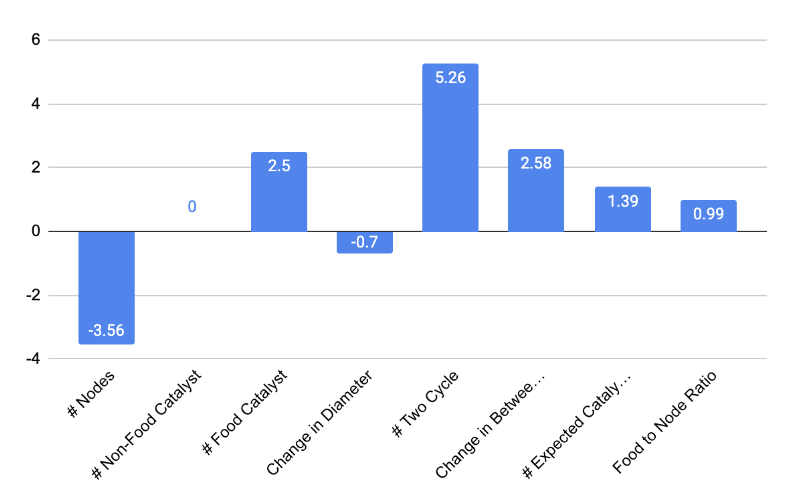
\includegraphics[width=15cm]{classification}
    \caption{Classification Results}
\end{figure}

Since we normalize the features before conducting the logistic regression, we cannot meaningfully apply the log-odds interpretation of logistic regression coefficients, but the relative differences between the values provides us insight into each features importance in predicting an RAF set.
From the chart it is clear that our three most prominent features are the number of two cycles, change in betweenness centrality, and number of food catalysts. 
Additionally, we see that the number of nodes is inversely related to the presence of an RAF set.  
Furthermore, we see that the number of two cycles is about twice as influential as either food catalysts or change in betweenness centrality.  

From our classification results it is apparent that proximity to the food set is important to finding RAF sets in the data. 
We also see that catalysts relations involving food set molecules are relatively more important than their counterparts.
Finally, we notice that two cycles, or self-autocatalytic reactions are incredibly important in producing an RAF set/subset.

\section{Stability}

\subsection*{Methodology}

From Hordjik and Steele's work we know that RAF probability can be modeled as a function of probability of catalyzation, but what makes different networks successful in producing an RAF for the same probability? 
We propose answering this question by introducing the notion of RAF stability. In other words, how does a network respond to a perturbation of either adding or removing an edge?
In the case that we do not have an RAF set in our network, our perturbation adds an arbitrary catalyzing edge to the set. 
On the other hand, if we do have an RAF set in our network, our perturbation acts to remove a random catalyzing edge from the set. 
After doing so, we can look at the percentage of networks that remain in their existing state and quantify the "stability" of the RAF set. 

Note that from our work with classification we see that proximity and catalysts from the food set are incredibly important in determining the presence of an RAF set. 
With this in mind, we act to test a second hypothesis using food-set perturbations.
In other words, each perturbation acts to either add/remove food-set catalysts where applicable. 

This simulation was conducted by finding an f value that produced approximately a 50\% probability of RAF and running repeated simulations of creating a network, testing whether it was RAF, applying the appropriate pertubration, and then seeing whether the new network exhibited an RAF set. 
A summary of the number of trials run for each value of n can be found below.

\begin{table}[h!]
    \centering
     \begin{tabular}{||c| c||} 
     \hline
     Max Molecule Size (n) & Number of Trials \\ [0.5ex] 
     \hline\hline
     2 & 5000 \\ 
     3 & 2500 \\
     4 & 1000 \\
     5 & 1000 \\
     6 & 500 \\
     7 & 300 \\ [1ex] 
     \hline
    \end{tabular}
\end{table}

\subsection*{Results and Analysis} 

\begin{figure}[H]
    \centering
    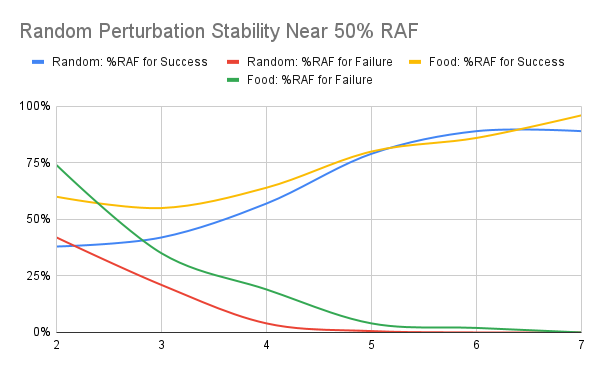
\includegraphics[width=15cm]{perturbation}
    \caption{Perturbation Results}
\end{figure}

As we can see here, as we increase n, the influence of the perturbation decreases. In other words, we can interpret this as a measure of large-autocatalytic network stability. 
We can also see that the food set perturbation is more influential than a random perturbation which corroborates our findings from the classification analysis. 
Furthermore, we can see that the influence of the food set perturbation is more pronounced at low n and levels off to match the random perturbation as n increases. 
It also appears that the random perturbation for success cases approaches an asymptotic bound, but more testing is needed to confirm whether this observation is a statistical artifact or representative of a deeper underlying phenomena.



\section{Conclusion}

Although this work does not prove or discover anything conclusive about the underlying structure and emergence of autocatalytic sets in prebiotic chemical models, my work this semester teases out interesting avenues for future research.
In particular, my work has found a strong correlation between graph properties, particularly proximity measurements between food set and the rest of the graph, and the presence of RAF sets. 
Although it is not conclusive at the moment, these results point us in the direction that the food-set may play a larger role in the emregence of RAF sets than previously considered. 
Similarly, the discovery of the importance of two-cycles in RAF sets may be indicitive of a model flaw, as two-cycles represent simple autocatalytic reactions.
If we are trying to model complex coupled autocatalytic reactions that exist in nature, relying on self-catalyzing reactions in the form of two-cycles may obscure our study of actual prebiotic autocatalytic emergence. 
Our perturbation analysis reveals to us that large kauffman networks are pretty stable under perturbations. In other words, if an autocatalytic set is able to be produced containing many molecules, it is difficult to disturb this set. 
In our understanding of prebiotic chemistry, this could indicate to us that the probabilistic bottleneck in autocatalytic reaction networks is not in the larger scale, but rather in smaller networks as the develop.



\section{Further Work}

In the coming semester I plan on taking a deeper dive into the ideas and critiques raised by my initial work this semester. 
In particular, I am interested in relaxing some of the model assumptions used in the Kauffman model to better replicate the real world.
As evidenced by the two-cycle classification result, if we control to remove the possiblity of two-cycles, we may be able to better understand the probabilistic limitations of RAF sets.
Also motivated by the classification portion of this project, I would like to better study how the expected number of food-set catalyzations correlates with RAF set prediction. 
In previous work we have seen expected number of catalyzations per molecule to be indicative of the probability of an RAF set, but given our results with food-set catalyzations, I am curious to see how this analysis would look under the lens of expected number of food-set catalyzations.
Finally, I would like to further test the stability of these RAF systems by continually perturbing the systems until we are able to change the state from RAF to no RAF or vice versa. 
In doing so, I hope to better understand the limits of stability and how this scales with network size.


\section{Acknowledgment}

I would like to thank Prof. Jun Korenaga for giving me the opportunity to work on this project. He has been an invaluable mentor and endlessly supportive throughout the process. 



\end{document}